\documentclass{article}
\usepackage[english]{babel}
\usepackage[letterpaper,top=2cm,bottom=2cm,left=3cm,right=3cm,marginparwidth=1.75cm]{geometry}
\usepackage{amsmath}
\usepackage{graphicx}
\usepackage[colorlinks=true, allcolors=blue]{hyperref}
\usepackage[utf8]{inputenc} % Required for inputting international characters
\usepackage[T1]{fontenc} % Output font encoding for international characters
\usepackage{listings}
\usepackage{color}

\definecolor{dkgreen}{rgb}{0,0.6,0}
\definecolor{gray}{rgb}{0.5,0.5,0.5}
\definecolor{mauve}{rgb}{0.58,0,0.82}

\lstset{frame=tb,
  language=Java,
  aboveskip=3mm,
  belowskip=3mm,
  showstringspaces=false,
  columns=flexible,
  basicstyle={\small\ttfamily},
  numbers=none,
  numberstyle=\tiny\color{gray},
  keywordstyle=\color{blue},
  commentstyle=\color{dkgreen},
  stringstyle=\color{mauve},
  breaklines=true,
  breakatwhitespace=true,
  tabsize=3
}
\begin{document}
\begin{titlepage}
	\newcommand{\HRule}{\rule{\linewidth}{0.5mm}} % Defines a new command for horizontal lines, change thickness here
	
	\center % Centre everything on the page
	
	%------------------------------------------------
	%	Headings
	%------------------------------------------------
	
	\textsc{\LARGE Fakultet Elektrotehnike i Računarstva}\\[1.5cm] % Main heading such as the name of your university/college
	\vfill
	\textsc{\Large Projekt R}\\[0.5cm]
	\textsc{\large Tehnička dokumentacija}\\[0.5cm] % Minor heading such as course title
	\HRule\\[0.4cm]
	{\huge\bfseries Sustav za procesiranje dokumenata pisanih pisaćom mašinom}\\[0.4cm] % Title of your document
	
	\HRule\\[1.5cm]
	
	%------------------------------------------------
	%	Author(s)
	%------------------------------------------------
	
	\begin{minipage}{0.4\textwidth}
		\begin{flushleft}
			\large
			\text{Student}\\
			Lovro Magdić
		\end{flushleft}
	\end{minipage}
	~
	\begin{minipage}{0.4\textwidth}
		\begin{flushright}
			\large
			\text{Nastavnik}\\
			Juraj Petrović
		\end{flushright}
	\end{minipage}
        \vfill\vfill\vfill\vfill\vfill\vfill\vfill\vfill\vfill
	{\large Siječanj 15, 2023.} % Date, change the \today to a set date if you want to be precise
	\vfill % Push the date up 1/4 of the remaining page	
\end{titlepage}

\section{Opis razvijenog proizvoda}
Cilj ovog projekta bio je razviti sustav za procesiranje dokumenata pisanih pisaćom mašinom. Sustav korisniku omogućuje lakše vizualno pregledavanje dokumenata, te računalno iščitavanje s dokumenata. Od korisnika očekuje se datoteka sa slikama nad kojima treba provesti procesiranje, sve ostalo sustav radi automatski. Odabir najboljih parametra, spremanje međurezultata, rotacija i slično.\\
\\
Cijeli proces obrade se odvija se kroz naredbeni redak odnosno u razvojnom okruženju po odabiru korisnika. Za razvijanje sustava korišten je Visual Studio Code (VSCode).\\
\\
Sustav je razvijen za python3 te zahtjeva razvojnu biblioteku openCV. OpenCV je biblioteka razvojnih funkcija za računalni vid u stvarnom vremenu,  njezine funkcionalnosti koristimo za razne obrade, spremanja i čitanja dokumenata.

\section{Opis rada sustava}

\subsection{Binary threshold i Image deskew}

U navedenom koraku koristimo navedene funkcije obrade: Binary threshold i Image deskew.\\
Threshold je segmentacijska funckija pomoću koje postižemo crno-bijelu sliku iz "grayscale" formata ili slike u boji. Preciznije za inicijalni threshold koristimo "Binary Threshold". Kao parametre prima granicu do koje nijanse sive postaju crne i iznad navedene granice nijanse sive postaju bijele. %ovdje umentni sliku Binary Threshold
\\
\begin{center}
    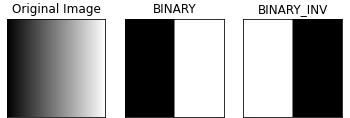
\includegraphics{binary_threshold.jpg}
\end{center}

Binary threshold nam omogućuje uklanjanje raznih artefakata koji bi otežali proces "Hough Line Transform".\\

Hough Line Transform je jednostvani transformacijski proces pomoću kojeg pronalazimo ravne linije na slici, u našem slučaju rubove papira na slici koja je prošla threshold. Nakon detekcije linija, računamo njihovu orijentaciju s obzirom na os apscise i time dobivamo kut zakrivljenosti. Navedeni kut odnosno kutevi nam olakšavaju postizanje uspravnosti papira na slici.\\

%ovdje stavi primjer sa neke slike di su nacrtane linije
Nakon određenog kuta zakrivljenosti preostaje nam rotacija slike. Za to koristimo definiranu funckiju "rotateImage" koja obavlja rotaciju pomoću integrirane funkcije "warpAffine" iz razvojne biblioteke openCV, slika se rotira oko svoga centra. %tu ubaci sliku koda rotateImage \\
\begin{lstlisting}
def rotateImage(cvImage, angle: float):
    newImage = cvImage.copy()
    (h, w) = newImage.shape[:2]
    center = (w // 2, h // 2)
    M = cv2.getRotationMatrix2D(center, angle, 1.0)
    newImage = cv2.warpAffine(newImage, M, (w, h), flags=cv2.INTER_CUBIC, borderMode=cv2.BORDER_REPLICATE)
    return newImage
\end{lstlisting}

Rotacija se ne provodi na slici koja je prošla threshold već na originalnoj slici, threshold sliku koristimo za izračun rotacije.
\begin{center}
    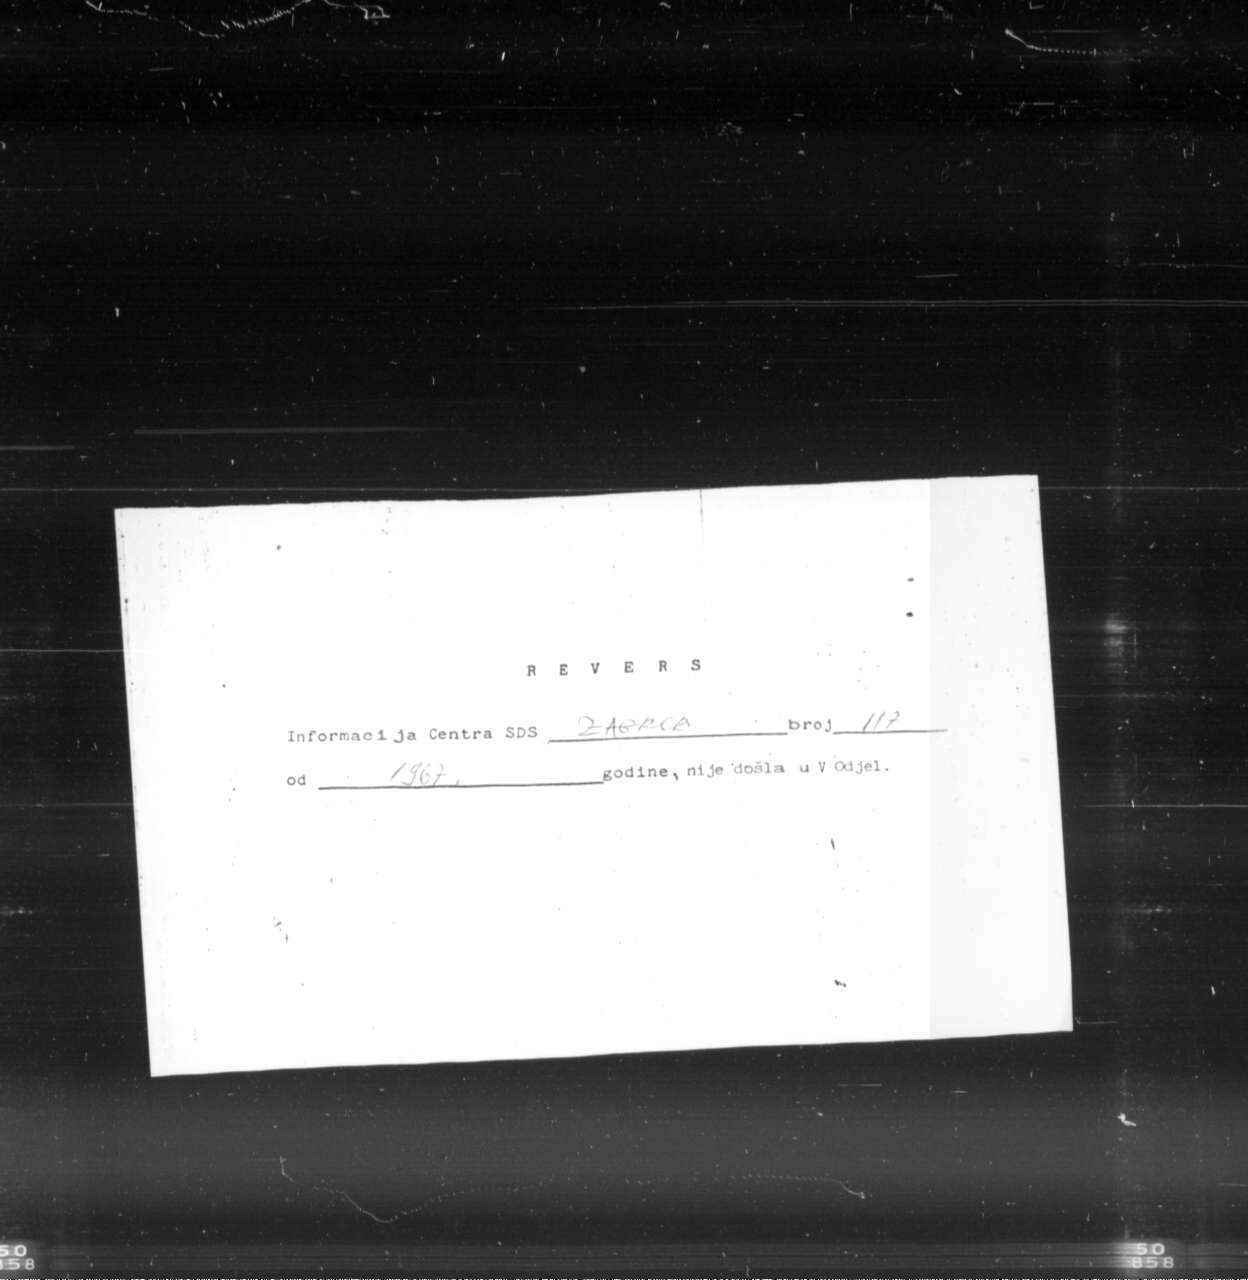
\includegraphics[scale=0.415]{Z05353721.jpg}
    
\includegraphics[scale=0.1]{Z05353721_draw.jpg}
    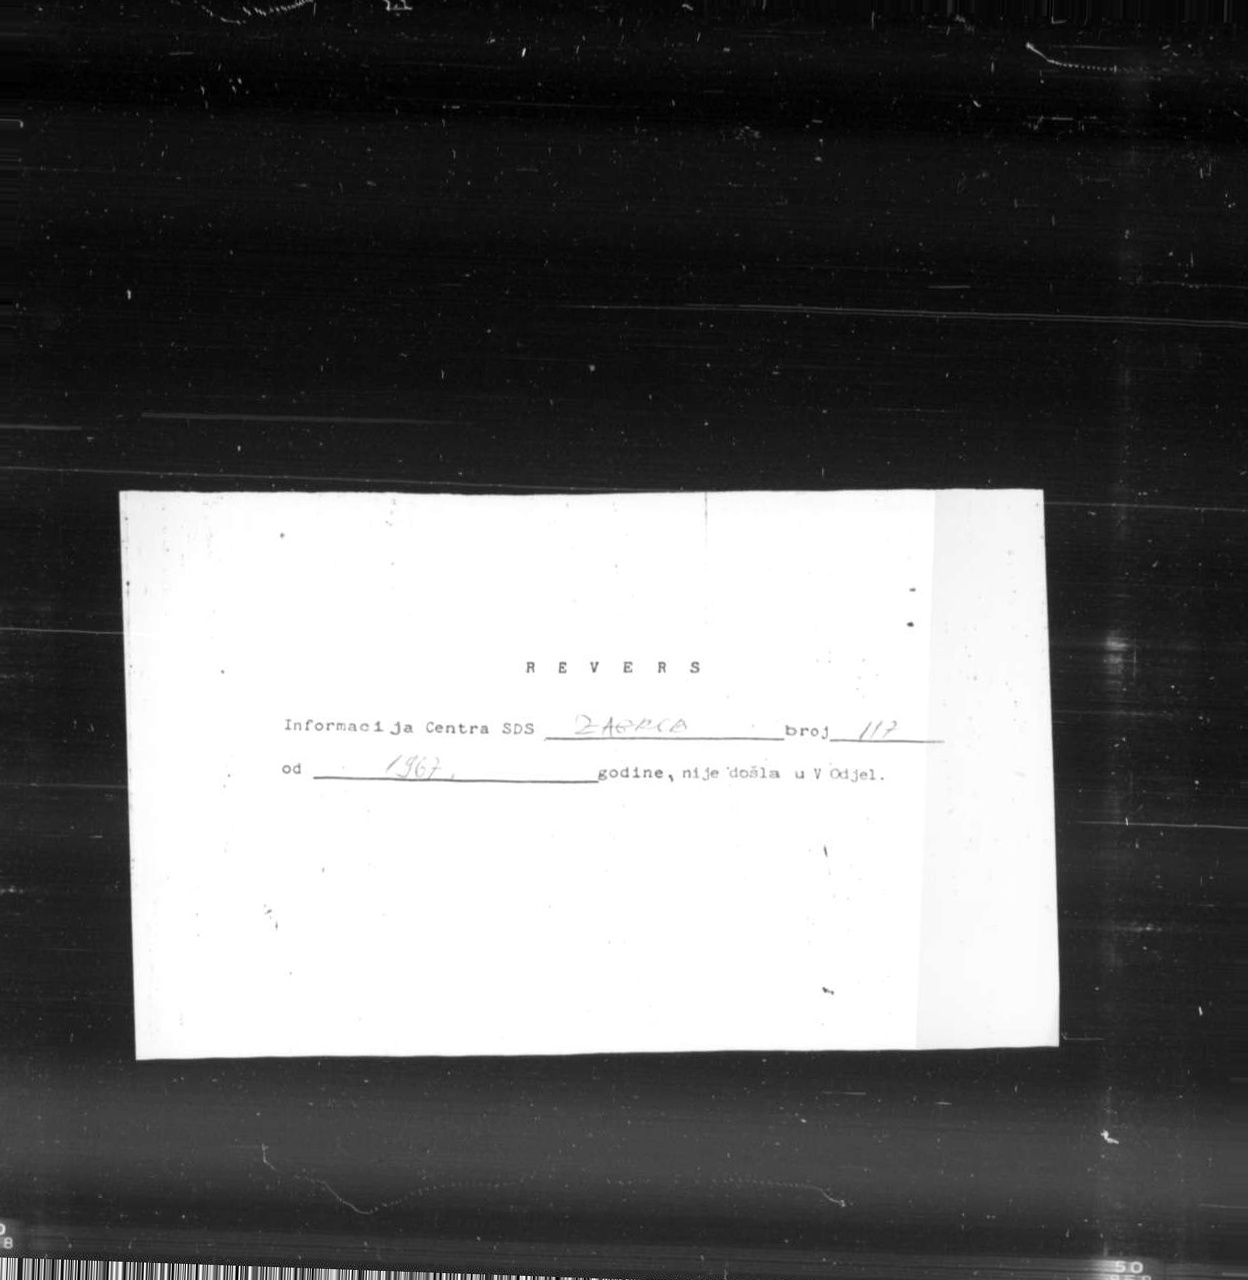
\includegraphics[scale=0.1]{Z05353721_deskewed.jpg}
\end{center}
%ubaci originalnu pored rotirane

\subsection{Contour detection}
Sljedeći korak u procesu obrađivanja slika je "contour detection". Bitan je za primjenu "adaptive threshold" funkcije i izuzimanje nepotrebnih artefakata iz slike (crne pozadine i artefakata). Radi na jednostavnom principu označavanja kontinuiranih točaka te lokaliziranje istih u skupinu odnosno konturu.\\ \\
Detekciju kontura provodimo na threshold slici a konture primjenjujemo na originalnoj odnosno rotiranom originalu.\\ %ubaci sliku sa konturom na originalu
\\
Kako bi postigli optimalnu konturu za svaku sliku provodimo detekciju optimalnog parametra threshold funkcije za svaku sliku.
Koristimo threshold u intervalu (100, 235) i računamo površinu konture koju je detektirao, određujemo razliku maksimalne konture i površine koju je sustav odredio za trenutni threshold. Optimalni threshold imat će najmanju razliku jer u tom slučaju imamo najprecizniju konturu stvarnom papiru na slici.
\newline
\begin{center}
    
\includegraphics[scale=0.15]{image_contour.jpg}
    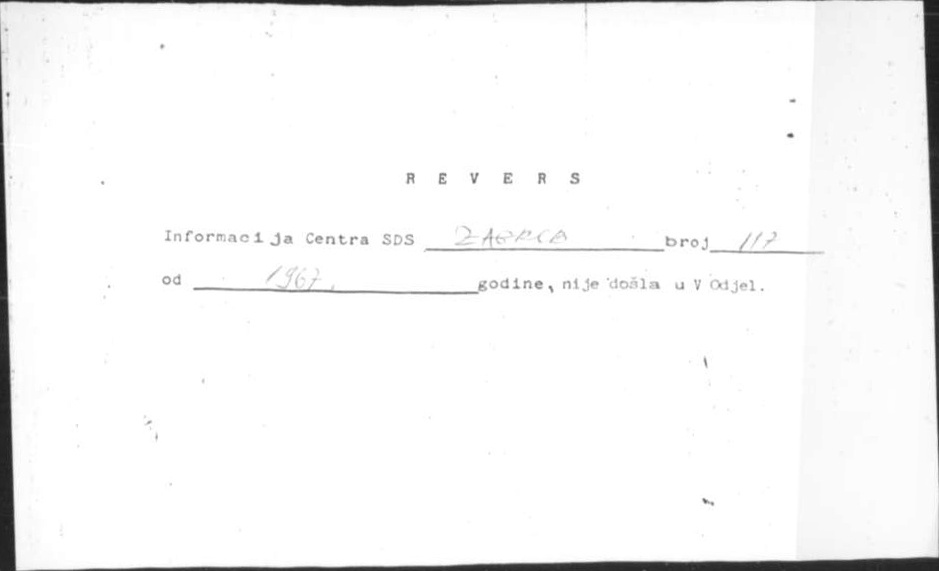
\includegraphics[scale=0.22]{Z05353721-cont.jpg}
\end{center}
\newpage
\begin{lstlisting}
for i in range(100, 235, 5):
        image = cv2.imread(each)
        img_gray = cv2.cvtColor(image, cv2.COLOR_BGR2GRAY)
        ret, thresh = cv2.threshold(img_gray, i, 255, cv2.THRESH_BINARY)

        contours, hierarchy = cv2.findContours(image=thresh, mode=cv2.RETR_TREE, method=cv2.CHAIN_APPROX_NONE)
        image_copy = image.copy()

        cv2.drawContours(image=image_copy, contours=contours, contourIdx=-1, color=(0, 255, 0), thickness=2, lineType=cv2.LINE_AA)

        c = max(contours, key = cv2.contourArea)
        x,y,w,h = cv2.boundingRect(c)

        ar.append([cv2.contourArea(c), w*h, i])
        array.append(int(w*h)-int(cv2.contourArea(c)))

    index = array.index(min(array))
\end{lstlisting}

\subsection{Gaussian blur}

Primjenom Gaussove funkcije u procesu zamućivanja slike smanjujemo detalje i šum prisutan na slici. Postignuti produkt nazivamo "Gaussian blur". %ubaci sliku gaussian blur
\begin{center}
    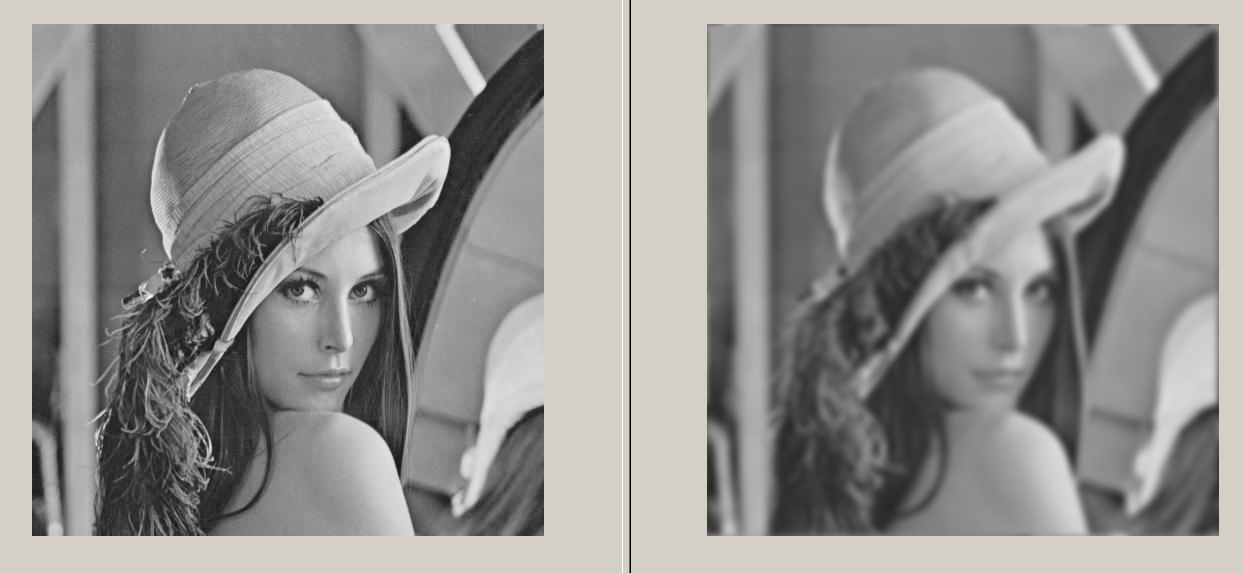
\includegraphics[scale=0.25]{gauss.png}
\end{center}

\subsection{Adaptive threshold}
Slike mogu sadržavati više razina različitog osvjetljenja i to
nam otežava određivanje optimalnog parametra thresholda. \\ Kako bi rješili taj problem koristimo funkciju "adaptive threshold" koja izračunava threshold parametar za piksele s obzirom na susjedne piksele. Time dobivamo različite vrijednosti thresholda za područja različitog osvjetljenja.
\newline
\begin{center}
    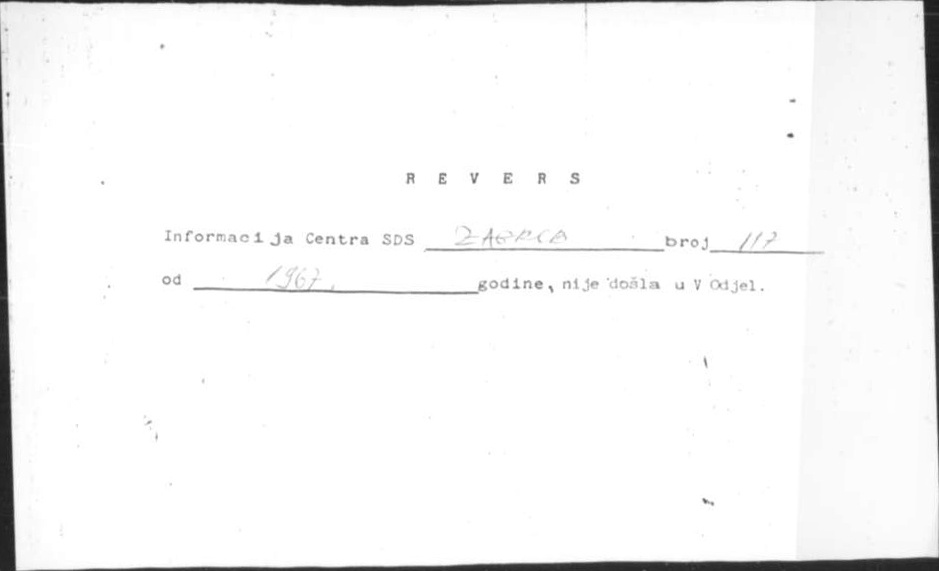
\includegraphics[scale=0.2]{Z05353721-cont.jpg}
    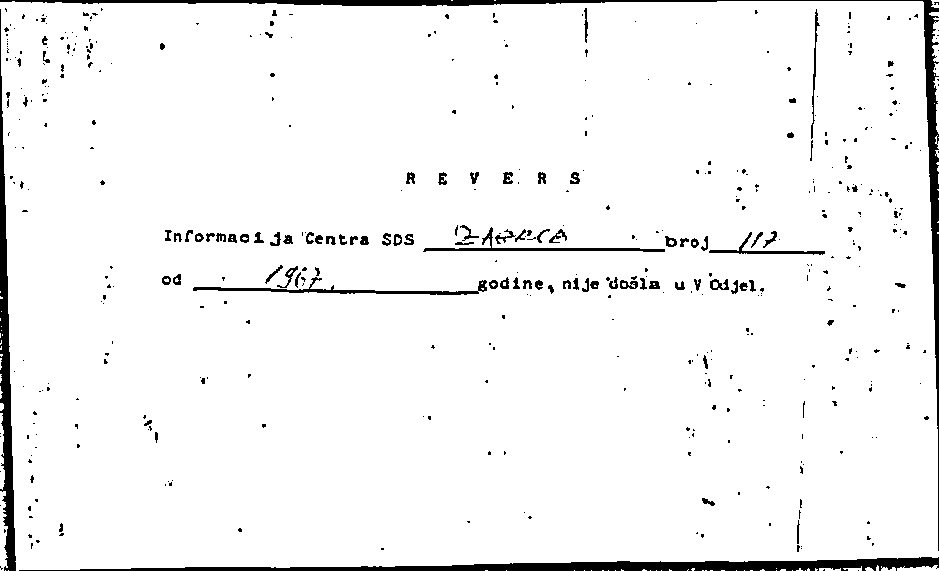
\includegraphics[scale=0.2]{Z05353721_adatpive.jpg}
\end{center}

\newline
\begin{lstlisting}
img = cv2.imread(each, 0)
image = cv2.adaptiveThreshold(img, 255,cv2.ADAPTIVE_THRESH_GAUSSIAN_C, cv2.THRESH_BINARY,25,4)
\end{lstlisting}

\subsection{Font thinning}

Kako bi olakšali optičko prepoznavanje znakova primjenjujemo proces stanjivanja fonta kojim također izbacujemo nepotreban šum oko znakova i postižemo detaljniju sliku. %ubaci primje stanjivanja i kod
\\

\begin{lstlisting}
def thin_font(image):
    image = cv2.bitwise_not(image)
    kernel = np.ones((2,1),np.uint8)
    image = cv2.erode(image, kernel, iterations=1)
    image = cv2.bitwise_not(image)
    return (image)
\end{lstlisting}
\\
\begin{center}
    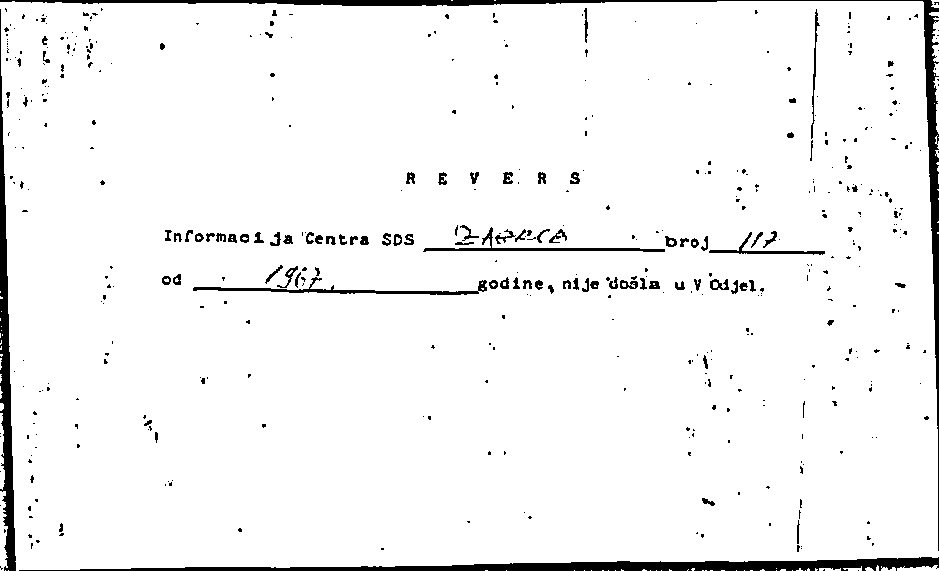
\includegraphics[scale=0.2]{Z05353721_adatpive.jpg}
    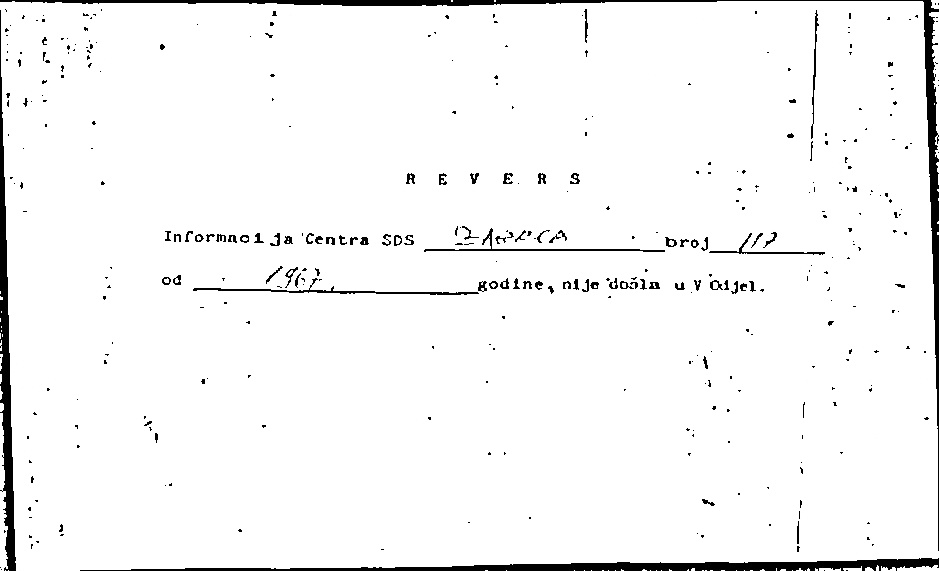
\includegraphics[scale=0.2]{Z05353721_thin.jpg}
\end{center}
\section{Upute za korištenje}
\\
Najnovija stabilna verzija dostupna je na \href{https://github.com/LovroMagdic/Image-preprocessing}{github-u}.
\begin{lstlisting}
git clone git@github.com:LovroMagdic/Image-preprocessing.git
\end{lstlisting}
\\
Sustav je razvijen za python3 te zahtjeva razvojne biblioteke openCV i Tesseract Python.
\begin{lstlisting}
pip install opencv-python
pip install pytesseract
\end{lstlisting}
\\
Nakon kloniranja repozitorija korisnik postavlja slike nad kojima želi provesti procesiranje u mapu "dataset" te pokreće "image\_preprocessing.py". Sustav automatski kreira preostale mape, rezultat obrade nalazi se u mapi "dataset\_final" odnosno isčitani podatci u "ocr". 
\newpage
\section{Literatura}
\end{document}